\section{Экспериментальные данные}

Резонанс ЛПП димеров исследовался с помощью микроспектроскопии пропускания. Схема экспериментальной установки показана на рис.~\ref{img:expsetup}.
\begin{figure}
\center{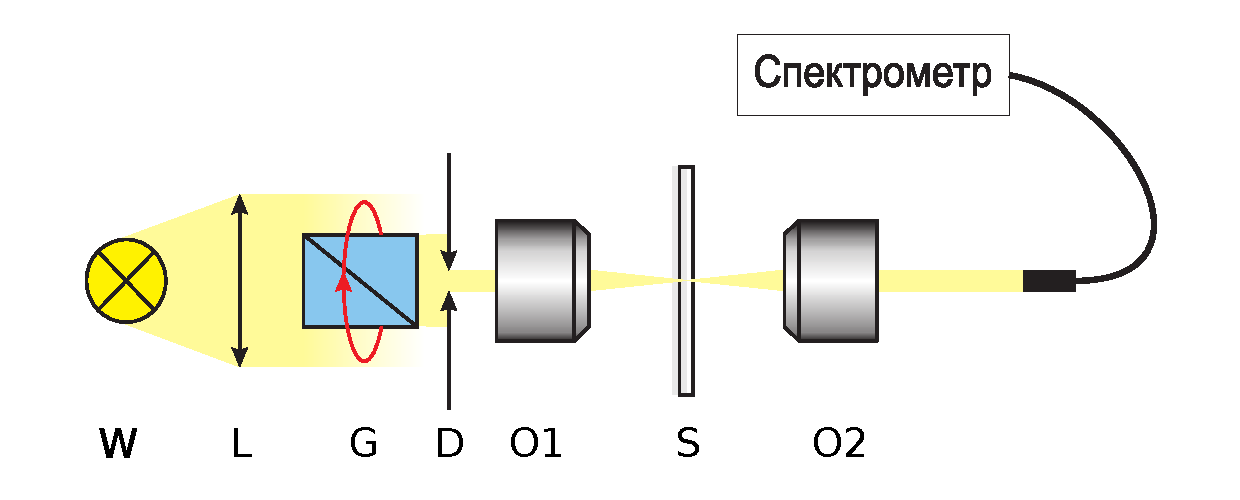
\includegraphics[width=12cm]{img/microspectroscopy/exp_setup.pdf}}
\caption{Схема экспериментальной установки. W --- источник света, L --- собирающая линза для формирования параллельного пучка света, G --- призма Глана-Тейлора для преобразования излучения в линейно поляризованное, O1, O2 --- система из двух объективов, S --- исследуемый образец. }
\label{img:expsetup}
\end{figure}
Спектры пропускания получались следующим образом: снимался спектр пропускания образца $ S_{sig} $, потом на расстоянии $ \approx 100 $ мкм от ансамбля димеров снимался спектр пропускания подложки $ S_{back} $. Конечный спектр пропускания $ S $ образцов определялся следующим образом:
\begin{equation}
S = \frac{S_{sig}}{S_{back}}.
\end{equation}
Для избавления от шумов каждая точка спектра сглаживалась по 15ти соседним с гауссовым весом. При определении положения резонанса выбиралась точка с минимальным коэффициентом пропускания, а также 10 соседних точек, и полученная кривая аппроксимировалась параболой $ y(x) = y_0 + (x - x_0)^2 $, где точка $ x_0 $ являлась положением резонанса ЛПП. Обработка данных производилась с помощью скрипта, написанного на языке программирования PYTHON. 

При получении спектров пропускания было выбрано два направления поляризации: параллельное наностержням и перпендикулярное им. При падении света с поляризацией, перпендикулярной наностержням, наблюдался небольшой сдвиг резонанса ЛПП в красную область спектра при уменьшении расстояния между наностержнями. И наоборот, при падении света с поляризацией, параллельной наностержням, наблюдался сдвиг в синюю область спектра при уменьшении расстояния между наностержнями. На рис.~\ref{img:Spectraa5d3} показан типичный спектр пропускания для света с поляризацией, параллельной наностержням. При этом наблюдается резонанс второго порядка, так как глубина модуляции составляет 5 \% и резонансная длина волны лежит не в инфракрасной области, как и в численных расчетах.
\begin{figure}
\center{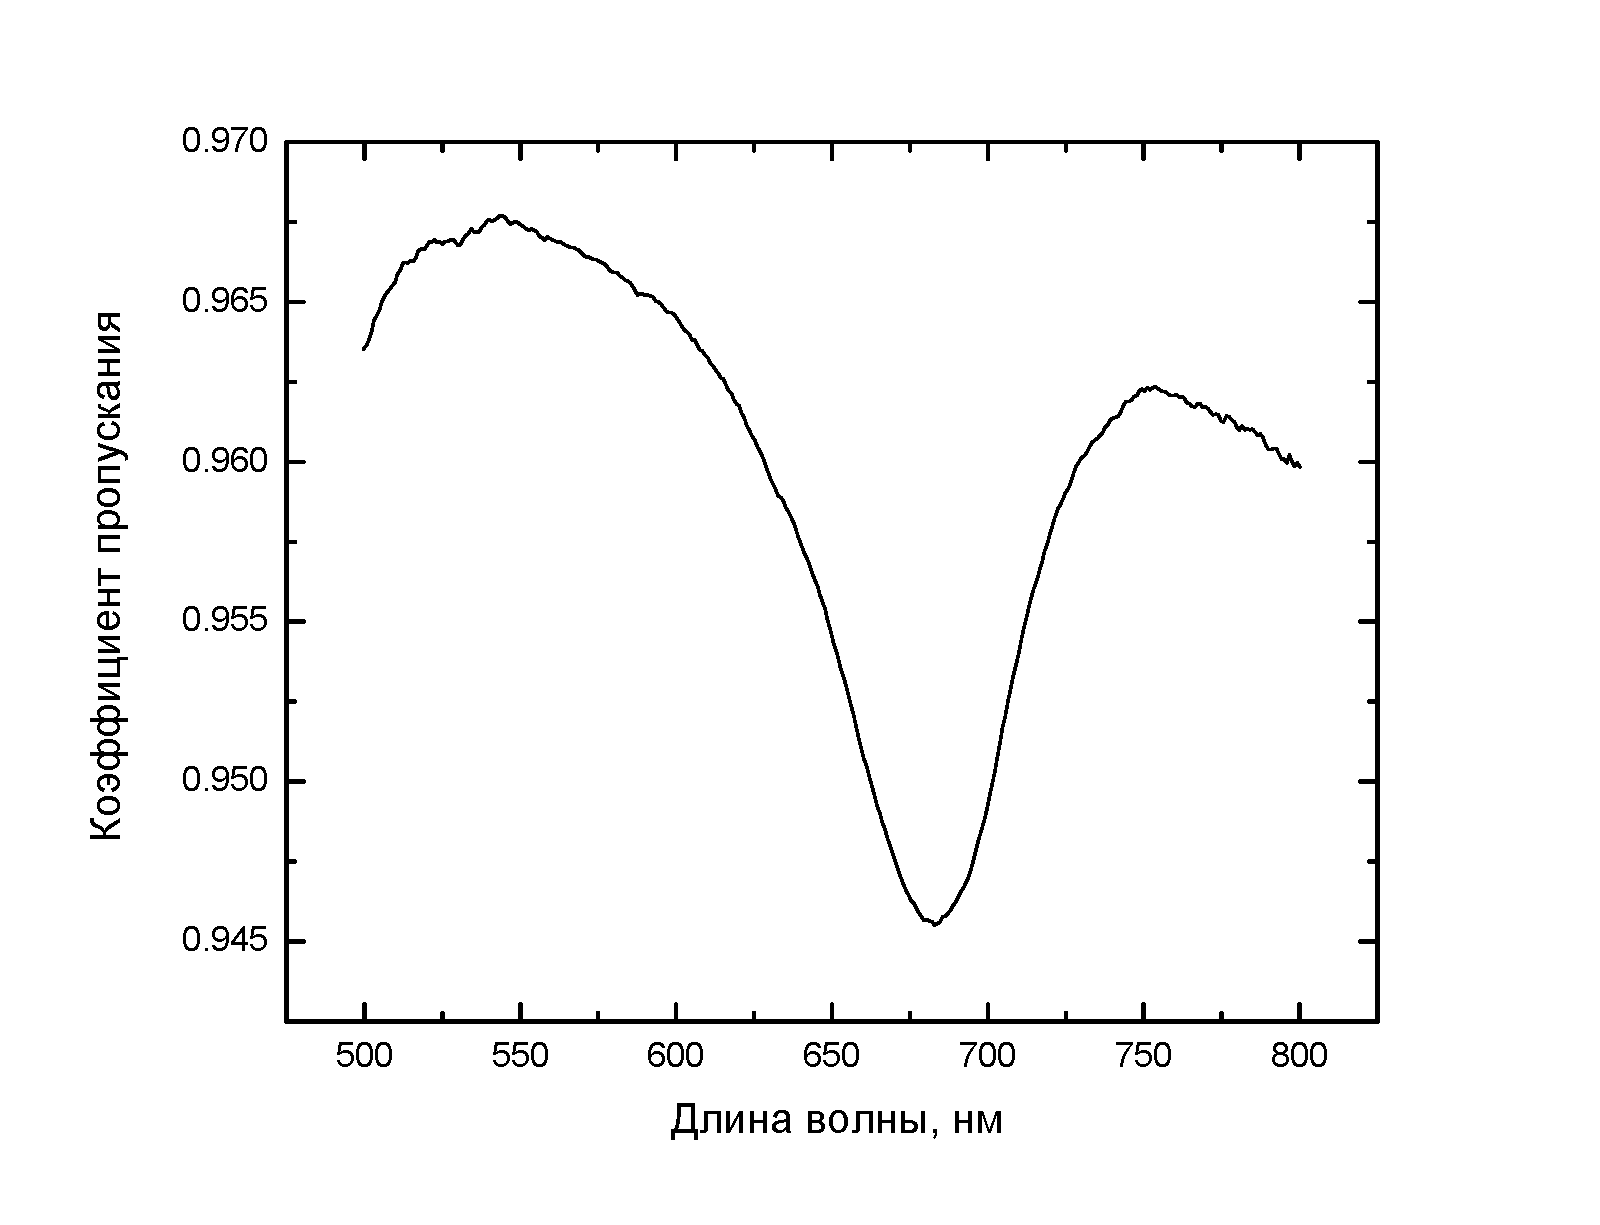
\includegraphics[width=10cm]{img/microspectroscopy/a400d300_spectra.pdf}}
\caption{Спектр пропускания ансамбля из наностержней с длиной 400 нм и расстоянием 250 нм между ними.}
\label{img:Spectraa5d3}
\end{figure}
На рис.~\ref{img:a500simexp} показана зависимость положения резонанса второго порядка как функция расстояния между наностержнями для длин наностержней 500 нм, рассчитанная численно (рис.~\ref{img:a500simexp}a) и полученная экспериментально (рис.~\ref{img:a500simexp}б). На экспериментальном графике нанесены систематические ошибки, которые рассчитывались следующим образом. Для фиксированного расстояния между наностержнями в 110 нм рассчитывалось численно положение резонанса второго порядка для длин наностержней 450 нм и 500 нм. Положение резонанса при этом составляло 685 нм и 713 нм. Так как погрешность в длине при изготовлении образцов составляла 3 нм, то систематическая ошибка определения положения резонанса ЛПП  $ \sigma_{err} \approx 2 $ нм. Видно, что абсолютные значения положения резонанса различаются в численном расчете и в эксперименте примерно на 100 нм. Это связано с тем, что численном расчете не учитывалась кварцевая подложка, которая влияет на положение резонанса ЛПП.
\begin{figure}
\center{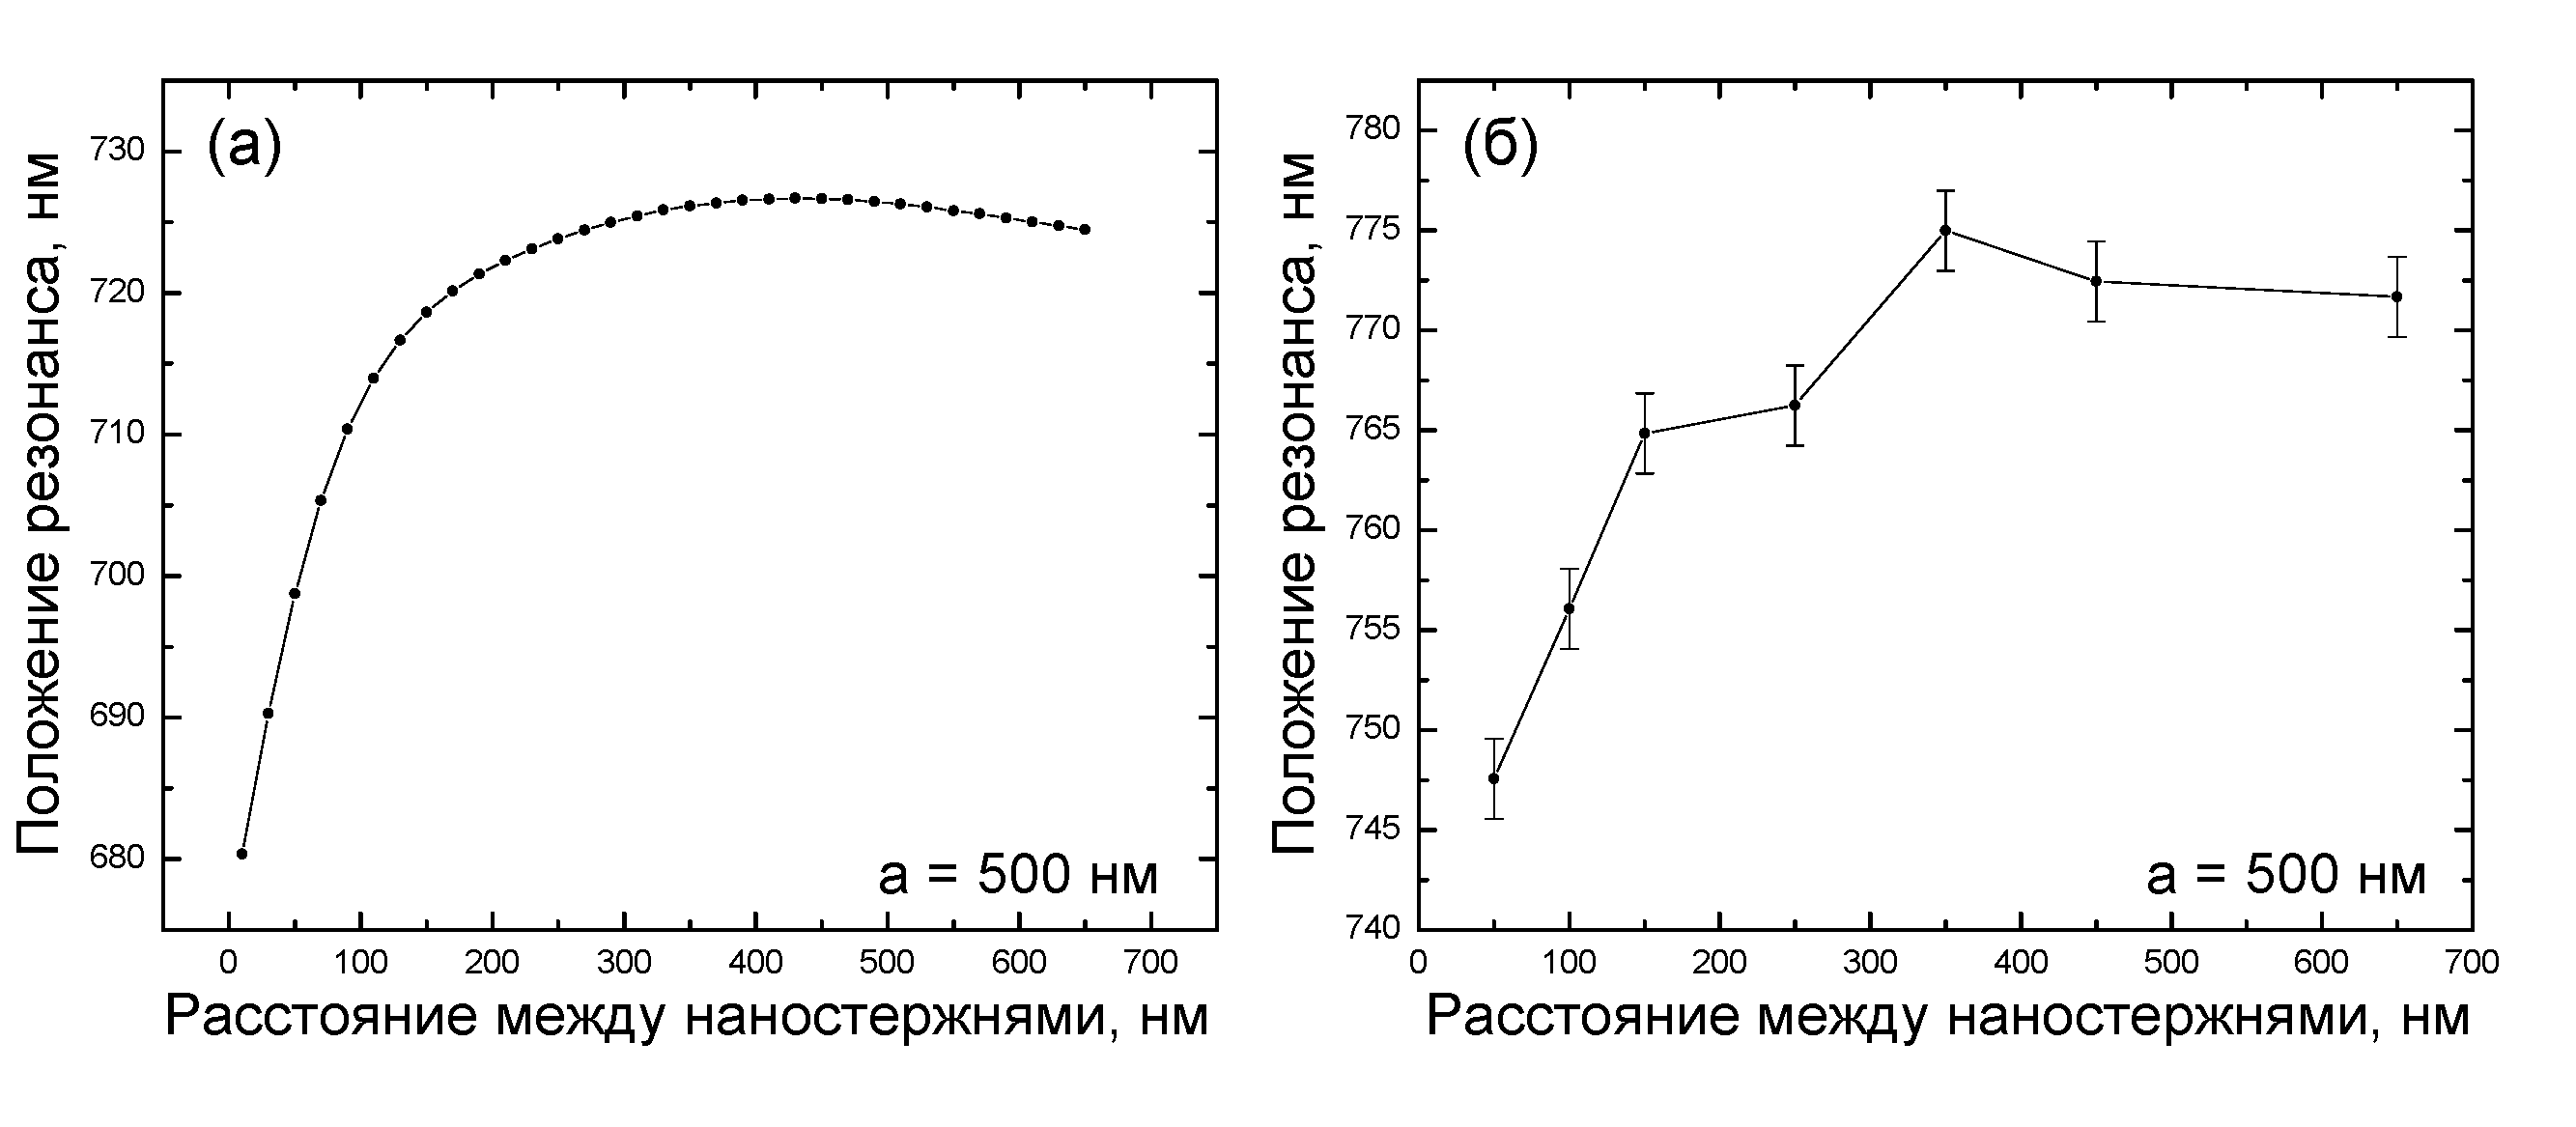
\includegraphics[width=16cm]{img/microspectroscopy/a500simexp.pdf}}
\caption{Рассчитанный численно (а) и полученный экспериментально (б) график зависимости положения резонанса второго порядка от расстояния между наностержнями для длин наностержней 500 нм. }
\label{img:a500simexp}
\end{figure}
\begin{figure}
\center{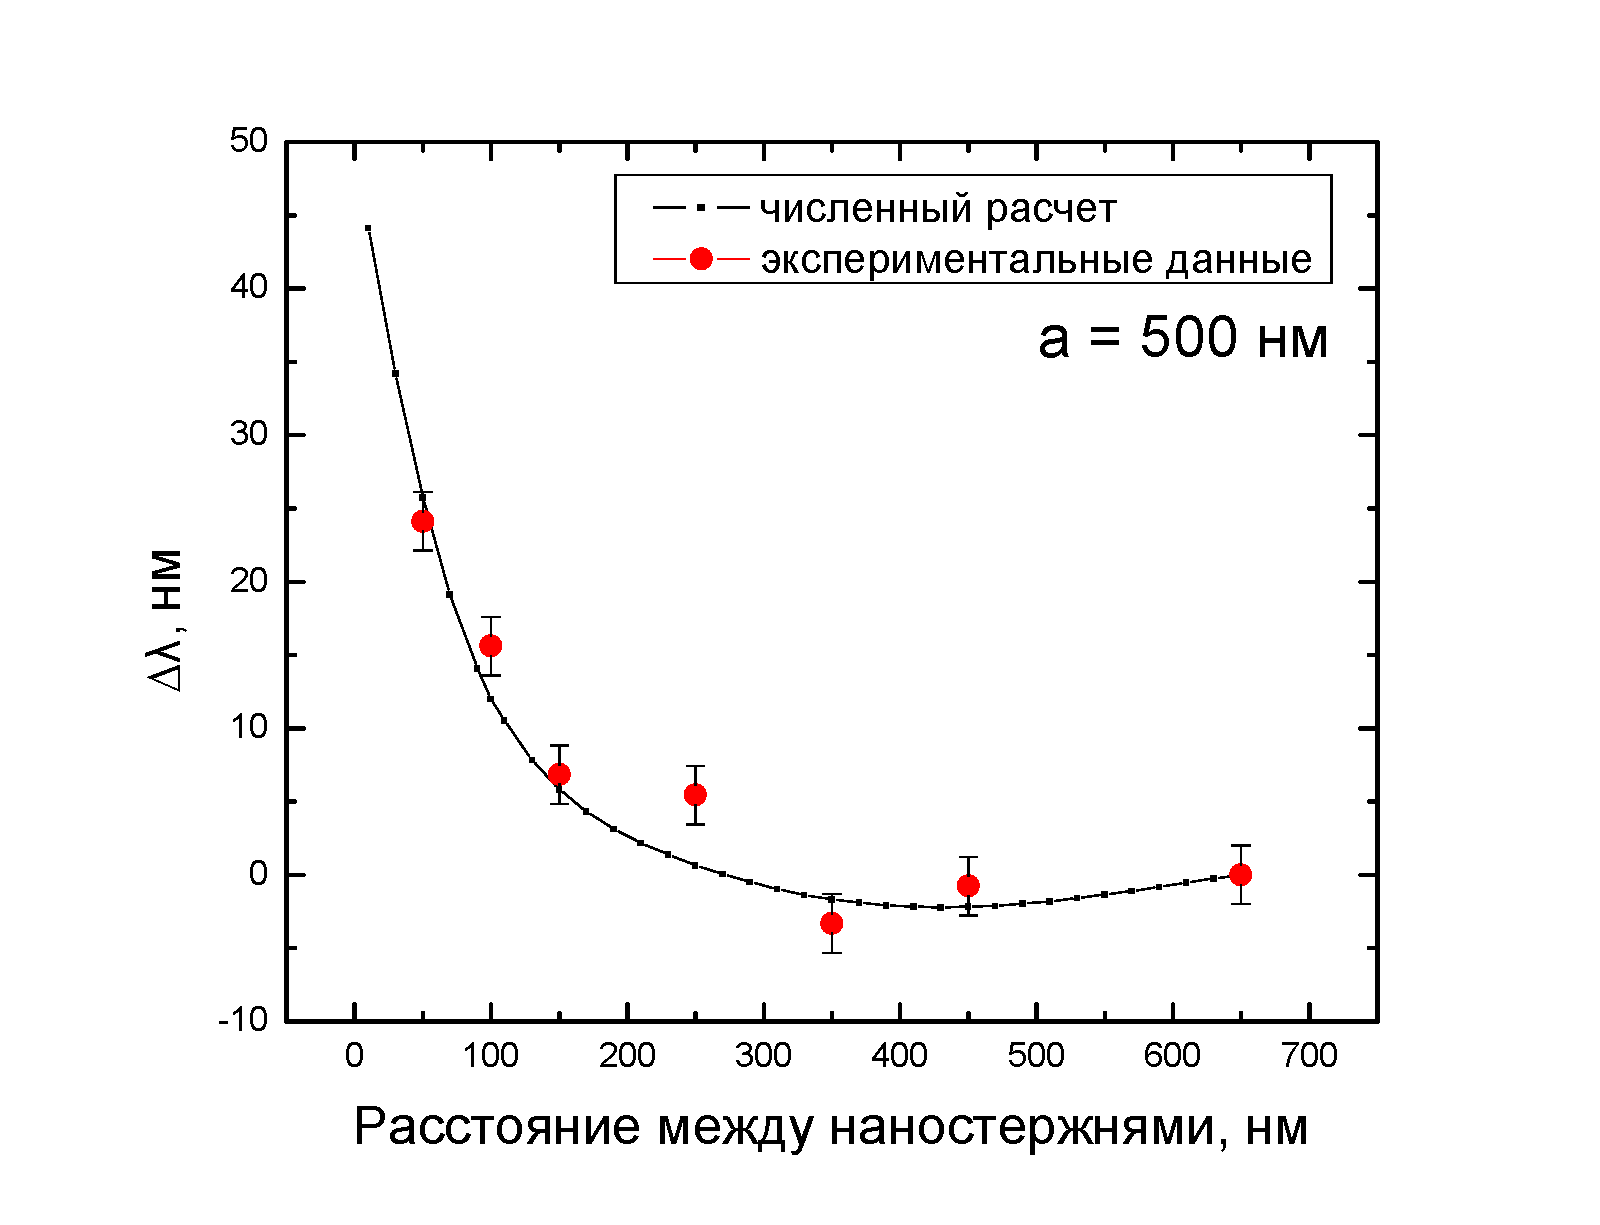
\includegraphics[width=10cm]{img/microspectroscopy/a500shift.pdf}}
\caption{График относительного сдвига резонанса второго порядка от расстояния между наностержнями при длине наностержней 500 нм.}
\label{img:a500shift}
\end{figure}

График относительного сдвига резонанса второго порядка показан на рис.~\ref{img:a500shift}. Здесь линией обозначены данные численного расчета, а красными точками -- экспериментальные данные. Видно, что численный расчет и экспериментальные данные сходятся в пределах погрешности за исключением точки, в которой расстояние между наностержнями составляет 250 нм. Это может быть связано с дальнепольным дифракционным взаимодействием, которое также влияет на положение резонанса.

Для пар наностержней длиной 400 нм также были получены численные и экспериментальные зависимости положения резонанса второго порядка от расстояния между наностержнями и  представлены на рис.~\ref{img:a400simexp}. Видно, что с уменьшением длины нанопалочек резонанс ЛПП сдвигается в синюю область. График относительного сдвига резонанса второго порядка от расстояния между наностержнями показан на рис.~\ref{img:a400shift}.
\begin{figure}
\center{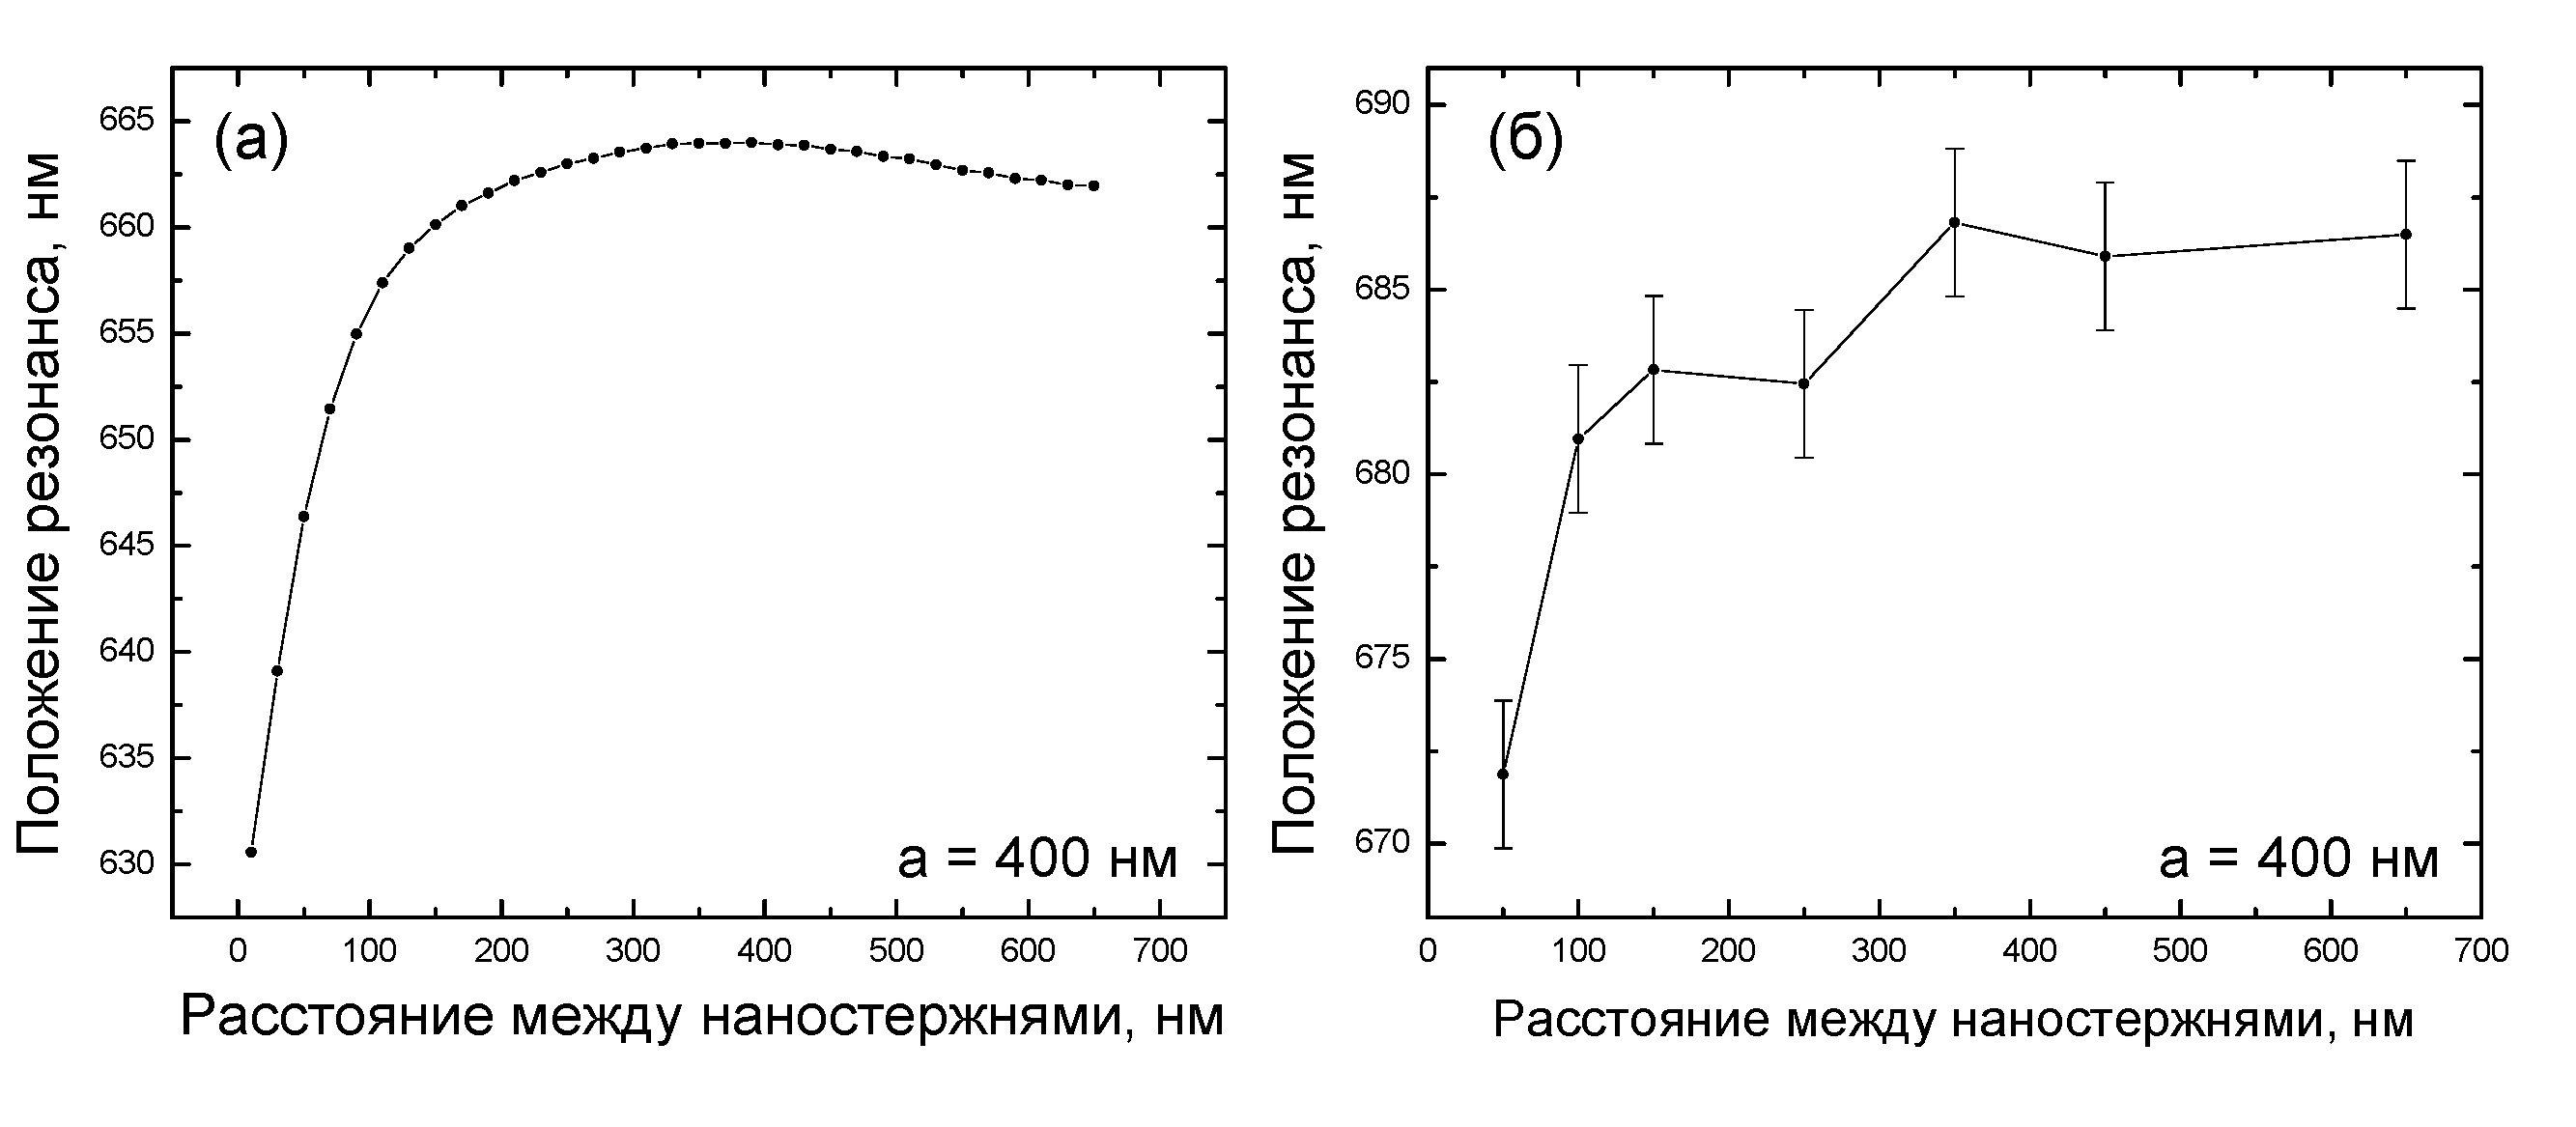
\includegraphics[width=16cm]{img/microspectroscopy/a400simexp.pdf}}
\caption{Рассчитанный численно (а) и полученный экспериментально (б) график зависимости положения резонанса второго порядка от расстояния между наностержнями для длин наностержней 400 нм. }
\label{img:a400simexp}
\end{figure}
\begin{figure}
\center{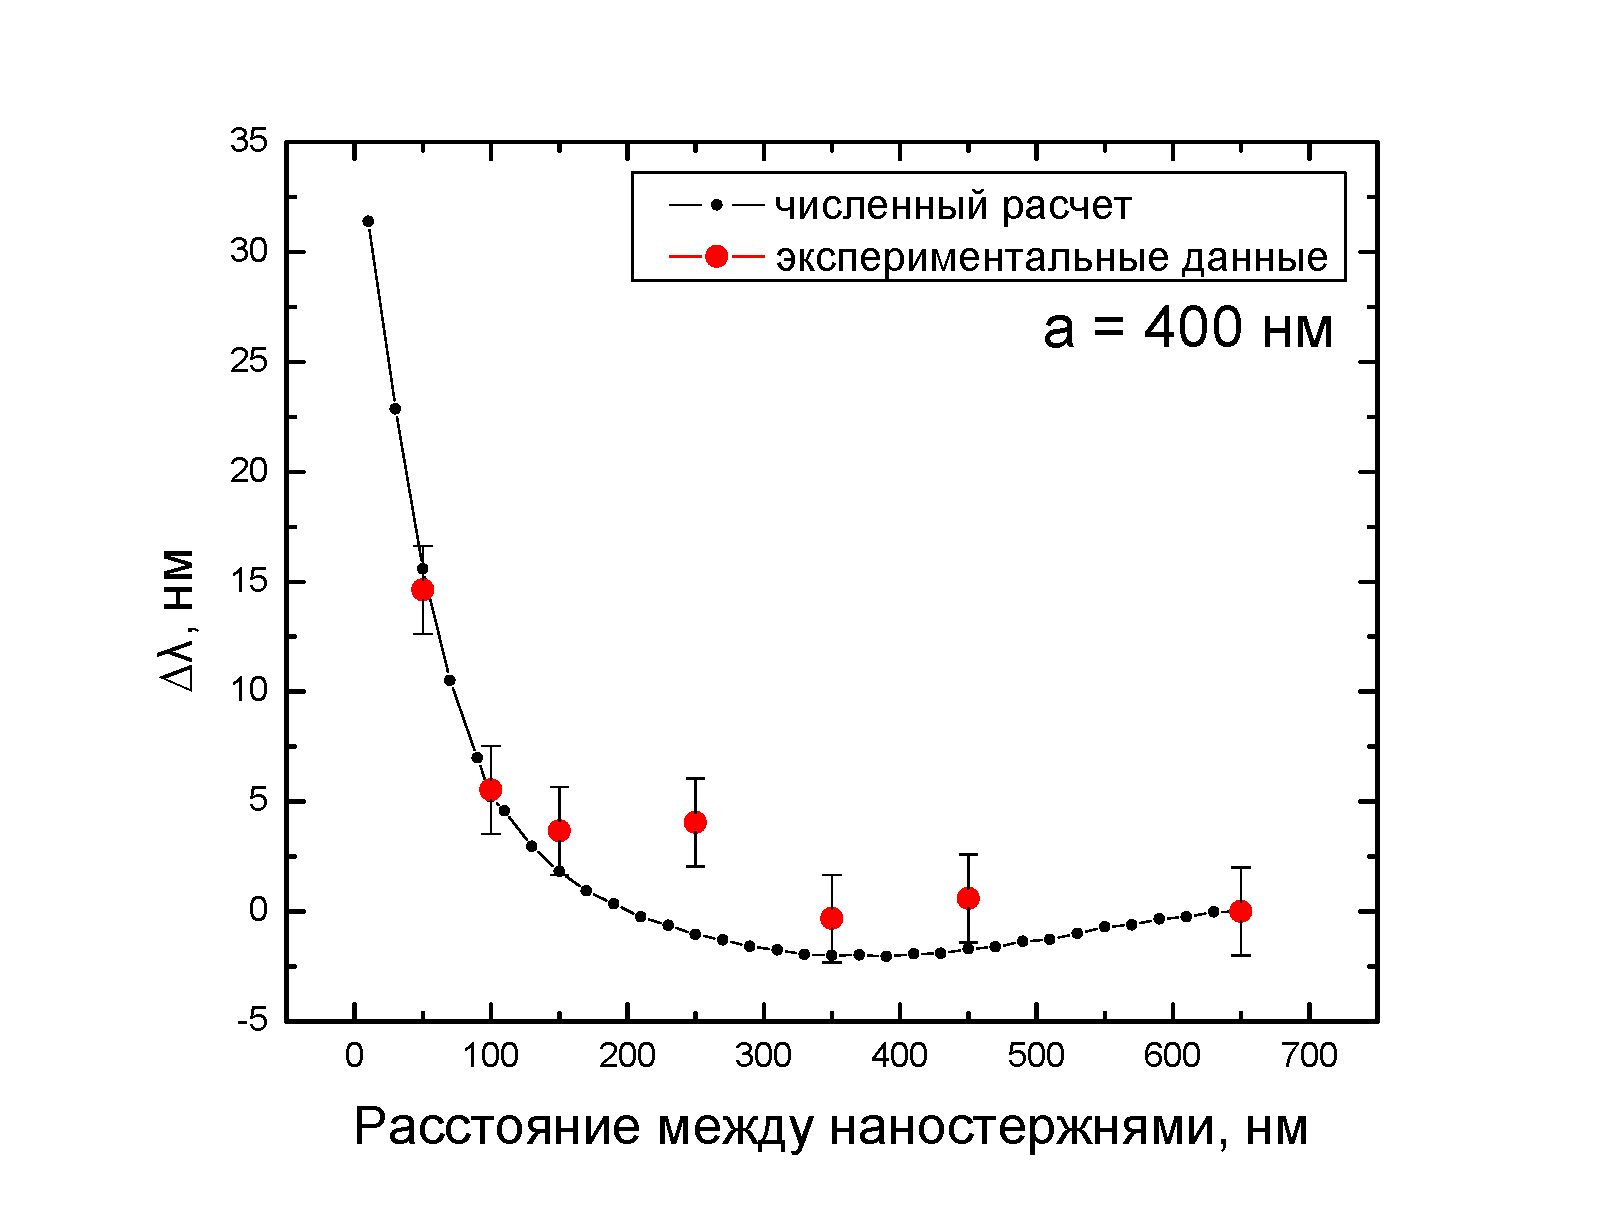
\includegraphics[width=10cm]{img/microspectroscopy/a400shift.pdf}}
\caption{График относительного сдвига резонанса второго порядка от расстояния между наностержнями при длине наностержней 400 нм.}
\label{img:a400shift}
\end{figure}
Такое поведение резонанса ЛПП хорошо согласуется с исследованиями систем димеров другой геометрической формы \cite{plasonrulereq, nanoprism}.

Далее исследовался спектр пропускания димеров с длиной 100, 150 и 200 нм. Характерный спектр пропускания для наностержней длиной 150 нм и расстоянием между наностержнями 100 нм показан на рис.~\ref{img:Spectraa1d1}. Глубина модуляции резонанса ЛПП составляет примерно 10 \%, а ширина на полувысоте резонанса ЛПП --- 100 нм. Для длин наностержней 150 нм данный резонанс является резонансом первого порядка.
\begin{figure}
\center{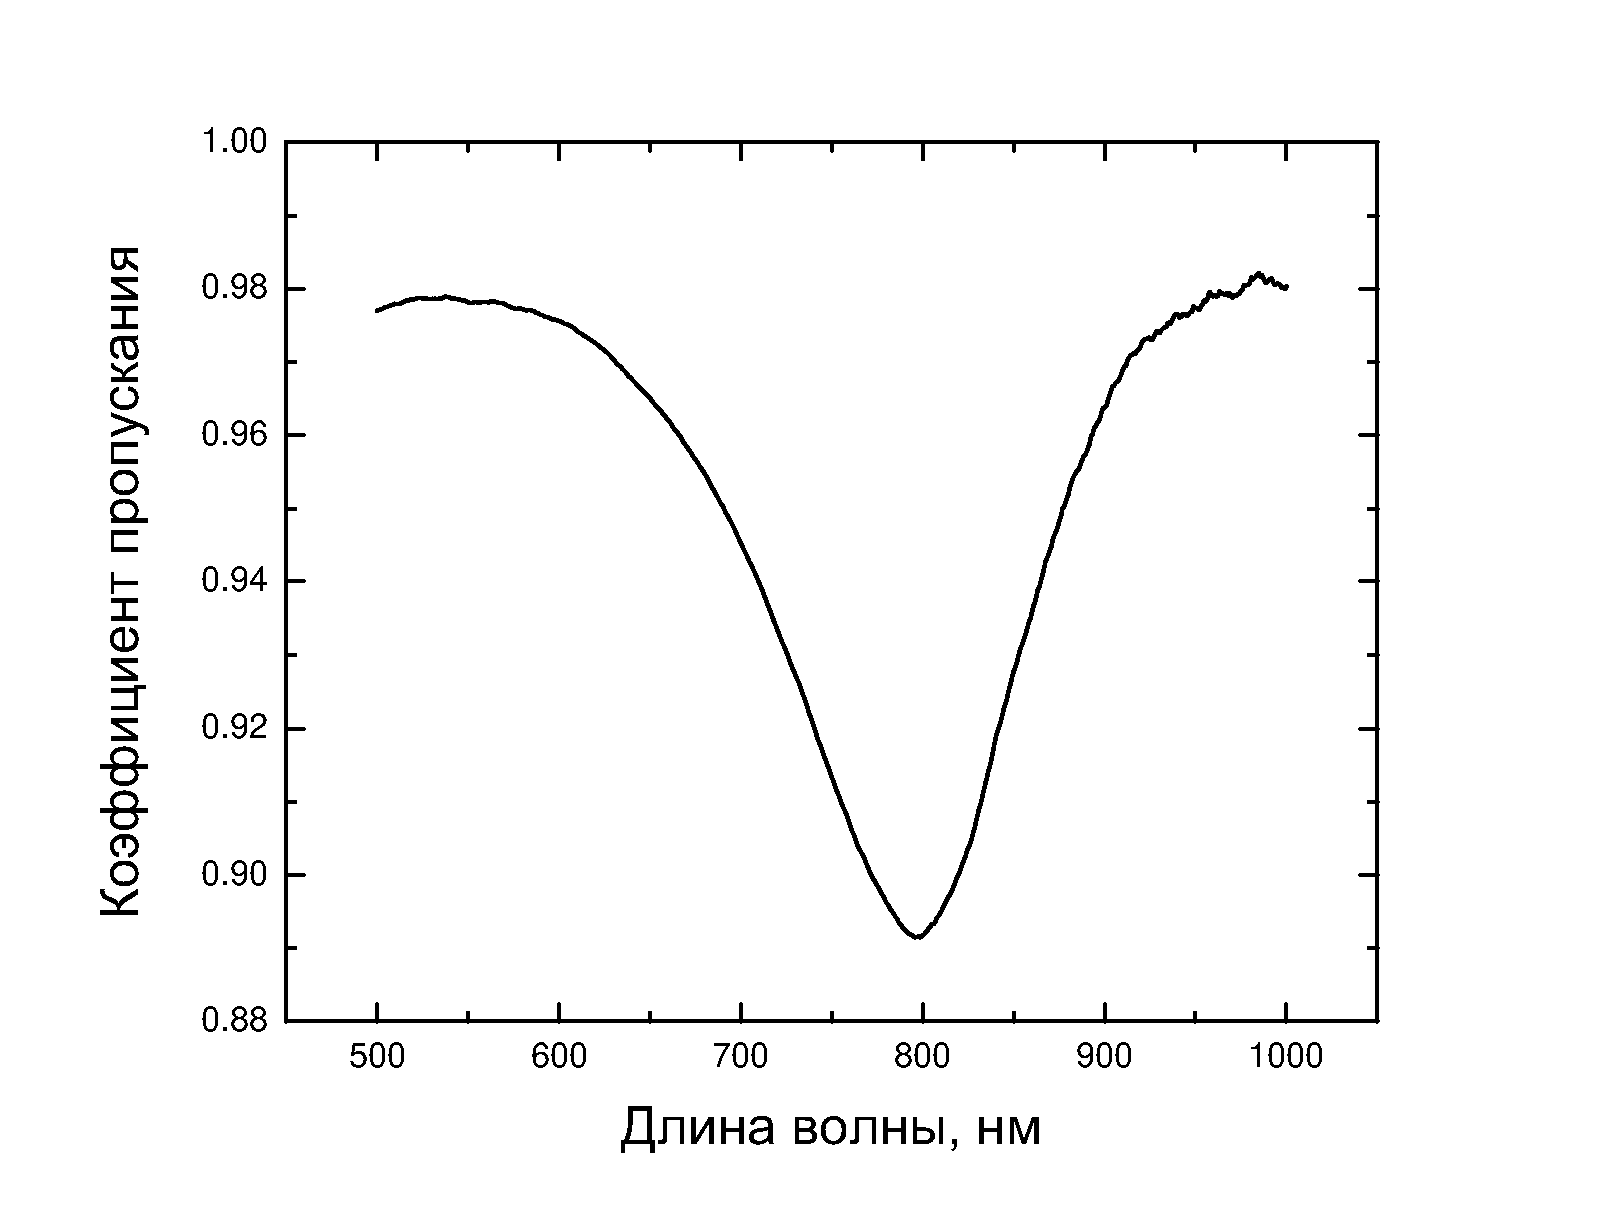
\includegraphics[width=10cm]{img/microspectroscopy/a150d100_spectra.pdf}}
\caption{Спектр пропускания ансамбля из наностержней с длиной 150 нм и расстоянием 100 нм между ними.}
\label{img:Spectraa1d1}
\end{figure}

На рис.~\ref{img:1res} показана зависимость резонанса первого порядка от расстояния между наностержней для длин наностержней 100, 150, 200 нм. Зависимость не носит характера насыщения, и наблюдаются осцилляции резонанса ЛПП первого порядка. Это связано, скорее всего, с дальнепольным взаимодействием наностержней, а также дифракционным взаимодействием между димерами, расстояние между которыми $ \approx 1$ мкм. Данные осцилляции являются паразитными для задачи построения <<плазмонной линейки>>, поскольку они мешают построению калибровочной кривой. Таким образом из экспериментальных данных следует, что для резонанса второго порядка возможно построить <<плазмонную линейку>> из-за его слабой чувствительности к дальнепольному взаимодействию, а для резонанса первого порядка влияние дальнопольного взаимодействия приводят к невозможности построения <<плазмонной линейки>>.
\begin{figure}
\center{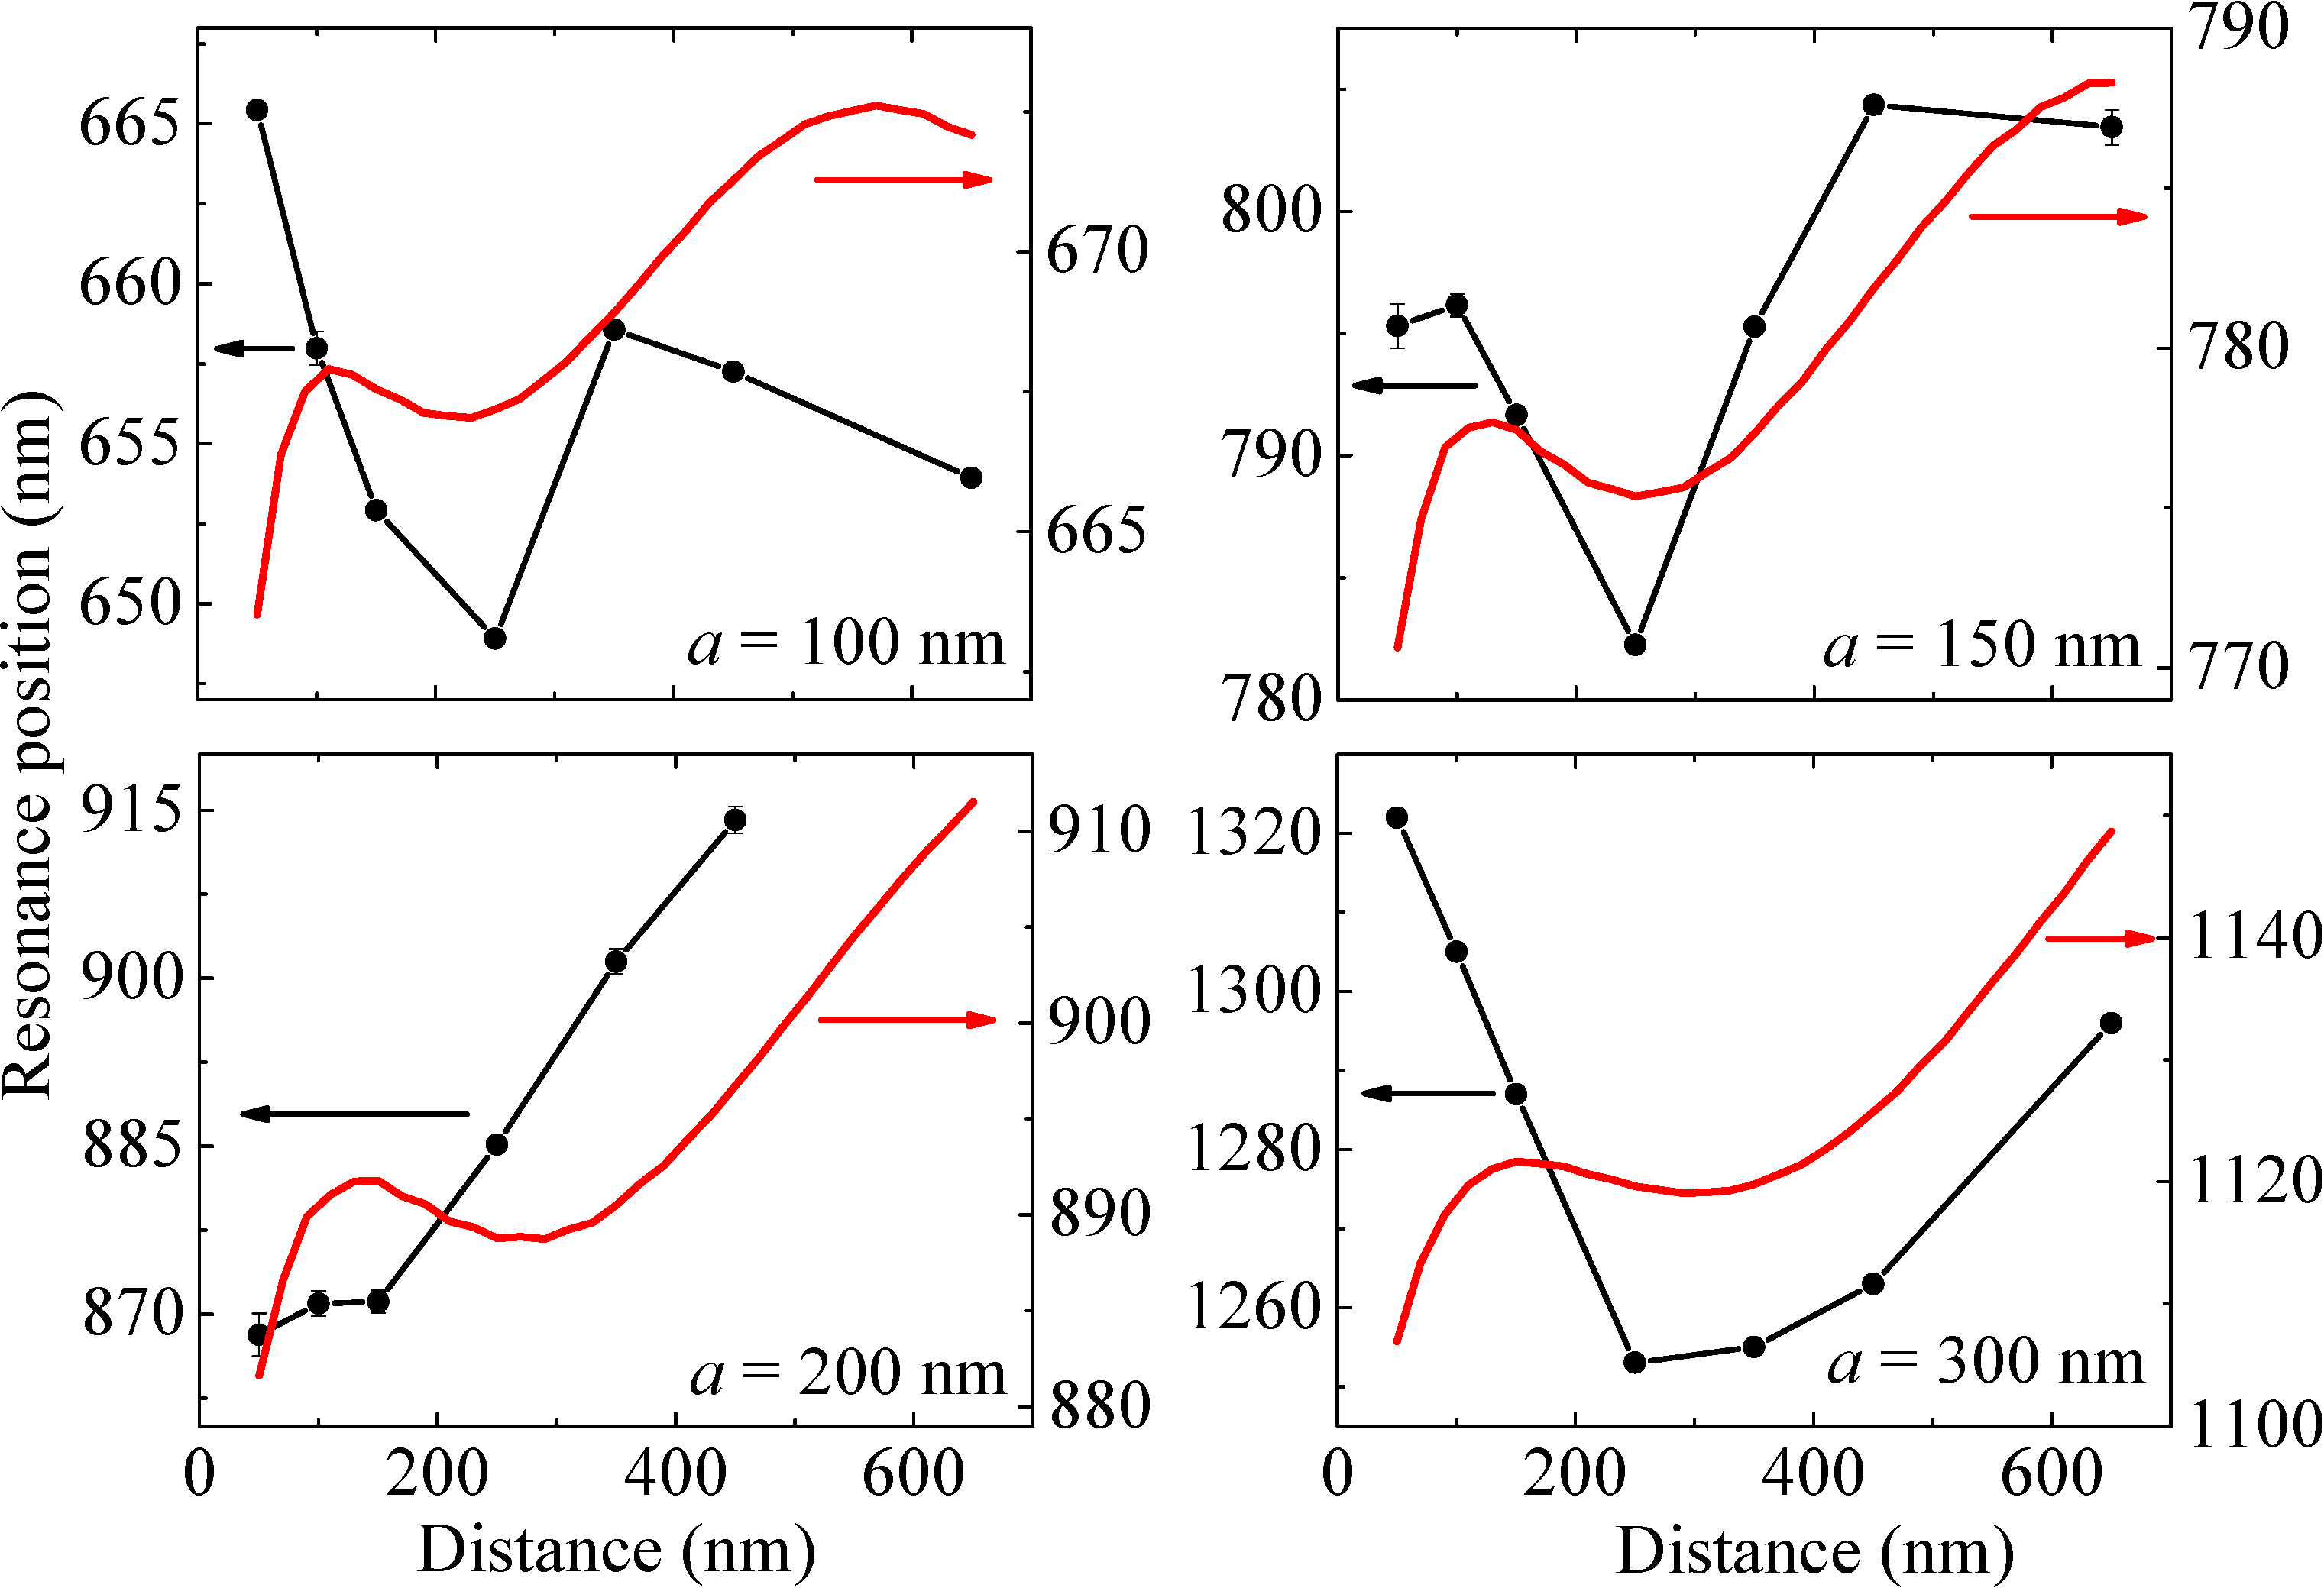
\includegraphics[width=18cm]{img/microspectroscopy/1res.pdf}}
\caption{Зависимость положения резонанса ЛПП первого порядка от расстояния между наностержнями при длине наностержней 100 нм, 150 нм и 200 нм.}
\label{img:1res}
\end{figure}

